\section{Empirical Results}

Report your findings. Use APA-style statistical reporting, e.g.,
a significant effect was found, $t(28) = 3.45$, $p < .001$, $d = 0.65$.
Regression estimates appear in Table~\ref{tab:empirical}, and
Figure~\ref{fig:empirical} shows the pattern of results.

% Generated by empirical/make_tables.R -- run empirical/main.R (or just
% that stage) to (re)build this table from empirical/data/processed/.
% Auto-generated by empirical/make_tables.R -- do not edit by hand.
\begin{table}
  \caption{Empirical Analysis: Regression Estimates}
  \label{tab:empirical}
  \begin{tabular}{@{}lrrrl@{}}
    \toprule
    Term & $B$ & $SE$ & $p$ & 95\% CI \\
    \midrule
    Intercept & 7.721 & 3.162 & 0.015 & [1.491, 13.951] \\
    $X_1$ & 0.369 & 0.060 & 0.000 & [0.250, 0.487] \\
    Treatment & 2.133 & 1.122 & 0.059 & [-0.077, 4.344] \\
    \bottomrule
  \end{tabular}
  \tablenote{$N$ = 233, $R^2$ = 0.154.}
\end{table}


% APA 7 figure: caption ABOVE the image, note below via \figurenote.
% Generated by empirical/make_figures.R.
\begin{figure}
  \caption{Outcome by Predictor and Group}
  \label{fig:empirical}
  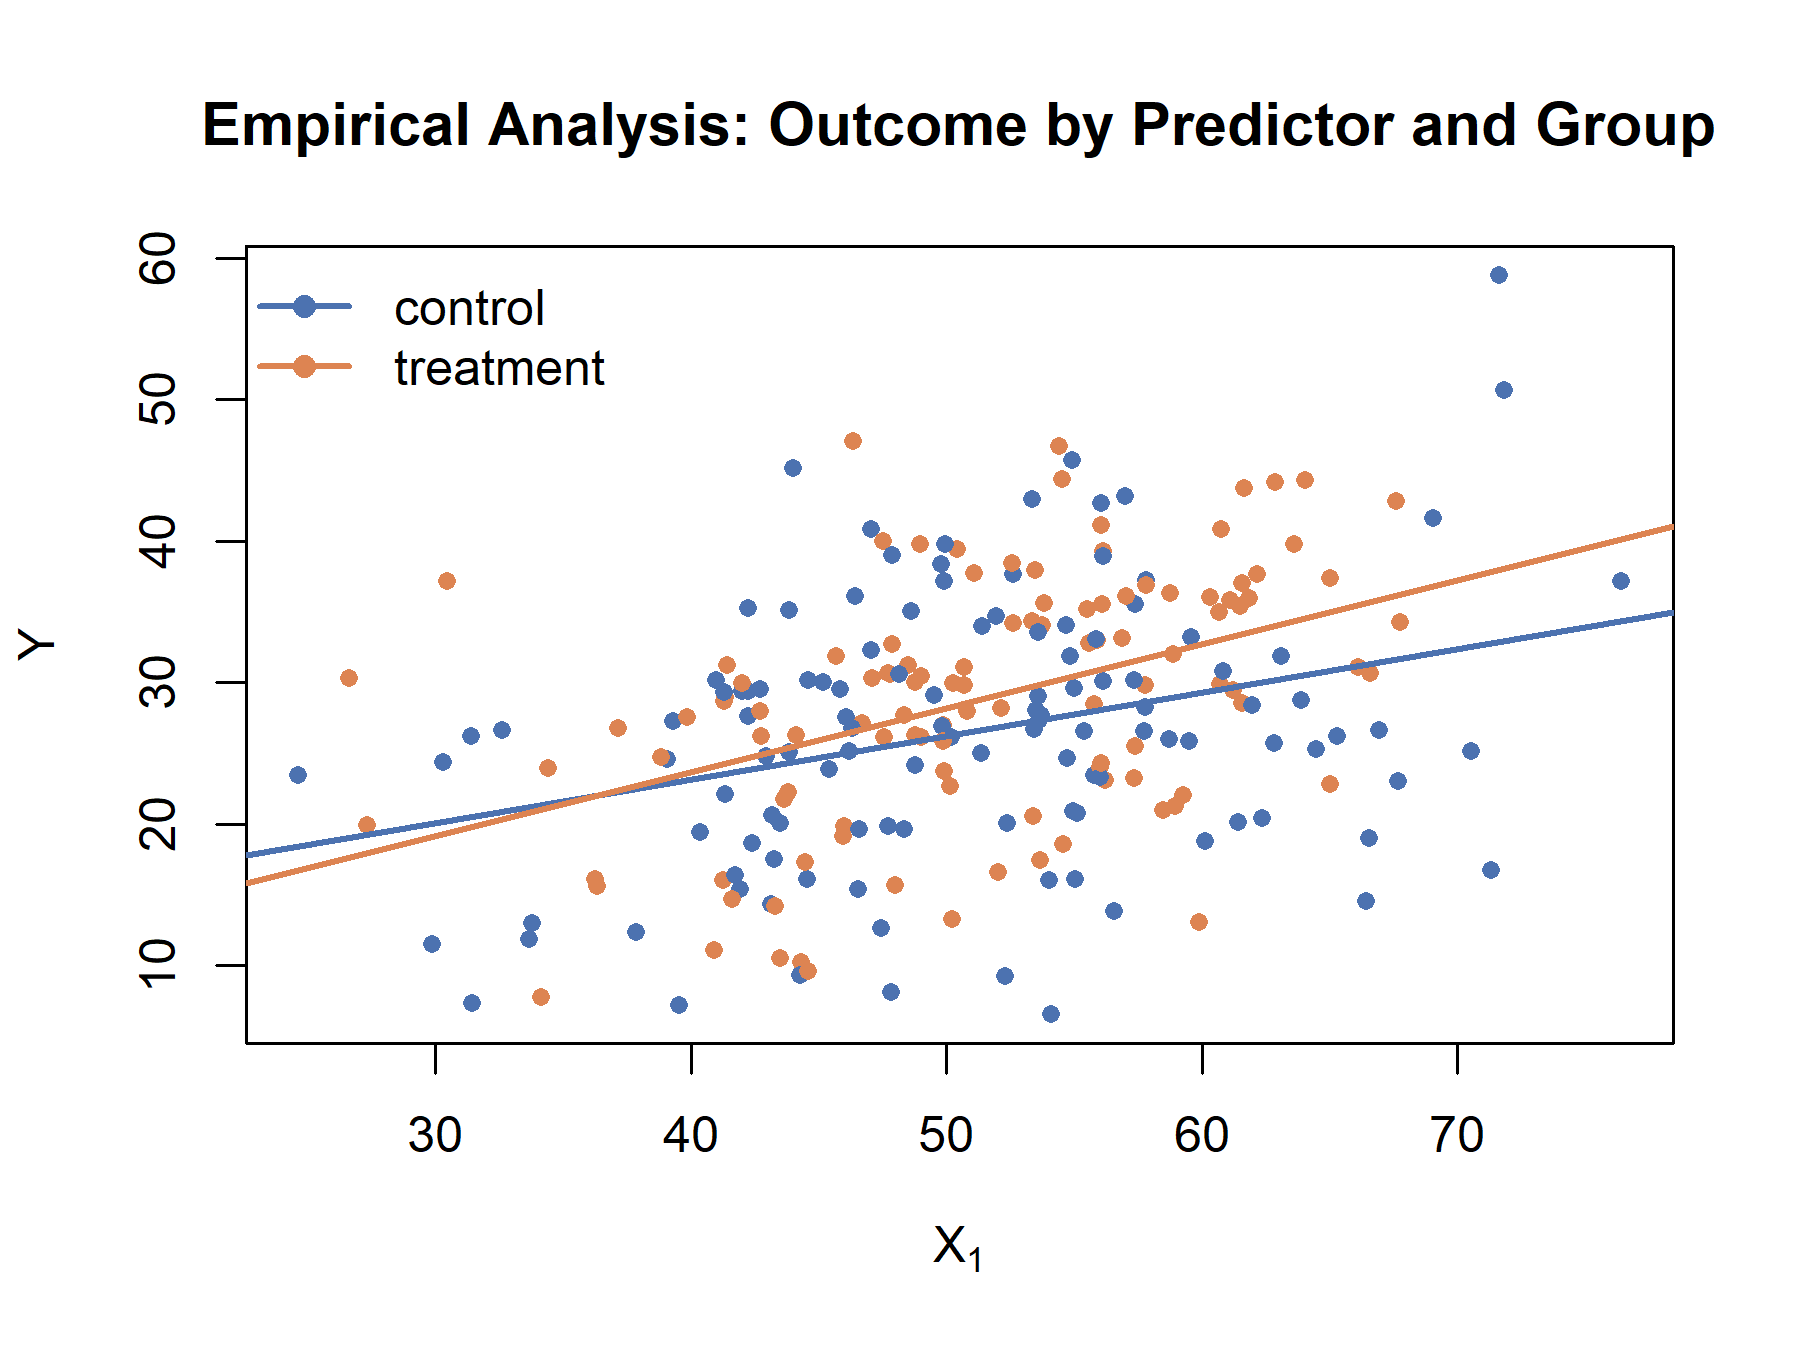
\includegraphics[width=0.7\textwidth]{empirical/figures/fig_empirical.png}
  \figurenote{Points are individual observations; lines are group-wise fitted values.}
\end{figure}
